\chapter{Методы формирования трехмерных микро- и наноструктур}

В настоящее время существует ряд областей, в которых является необходимым формирование трехмерных микро- и наноструктур -- микро- и наноэлектромеханических систем, дифракционных оптических элементов, микро- и наноканалов и др. Для решения этой задачи были разработаны различные методы -- как принципиально новые, так и основанные на методах формирования бинарного микрорельефа. В первой части данной главы описаны основные существующие методы микро- и наноструктурирования, а также их преимущества и недостатки. Вторая часть главы посвящена описанию перспективного, но в настоящее время еще не достаточно хорошо изученного метода -- сухого электронно-лучевого травления резиста.

\section{Основные методы микро- и наноструктурирования}

\subsection{Наноимпринтная литография}
Наноимпринтная литография (НИЛ) -- технология, предназначенная для переноса изображения наноструктуры или электронной схемы на полимерный материал путем прямого воздействия на него специальным штампом~\cite{NIL_1, NIL_2}.
Существуют два основных метода НИЛ -- термическая и ультрафиолетовая (УФ).
В термической НИЛ штамп вдавливается в слой полимера, нагретого до температуры, превышающей температуру стеклования полимера, затем происходит охлаждение полимера и извлечение штампа (рисунок~\ref{fig:NIL}a).
В ультрафиолетовой НИЛ штамп из материала, прозрачного в УФ части спектра, погружается в жидкий полимер, который отверждается под действием УФ излучения, после чего происходит извлечение штампа (рисунок~\ref{fig:NIL}б).
Штампы обычно изготавливается с помощью электронно-лучевой литографии из металла или кремния для термической НИЛ, и из полимеров или кварца -- для УФ НИЛ.
Учитывая прямой контакт штампа с основным материалом, а также масштаб печати 1:1, к плоскопараллельности и бездефектности штампа предъявляются высокие требования.
Перед проведением процесса НИЛ на штамп наносится специальное антиадгезионное покрытие, что позволяет избежать прилипания полимера к штампу при его отделении.
Также после процесса НИЛ на штампе неизбежно остается тонкий остаточный слой полимера, который удаляют с помощью плазменного травления.
Несмотря на то, что технология НИЛ изначально создавалась как альтернатива фото- и электронно-лучевой литографии, она может применяться для получения трехмерных микро- и наноструктур, таких как фотонные кристаллы~\cite{NIL_nanophotonics}, микроканалы~\cite{NIL_microfluidics} и \linebreak др.~\cite{NIL_3D_1, NIL_3D_2}.
Преимуществами НИЛ являются относительная простота процесса (при наличии штампа), высокая производительность и возможность достижения высокого разрешения (менее 100 нм).
К недостаткам этого метода относятся трудоемкость и дороговизна процесса изготовления штампа надлежащего качества, необходимость его частого обслуживания, сложность совмещения штампа с низлежащим слоем и ограниченный ресурс штампа.

\begin{figure}[t]
	\centering
	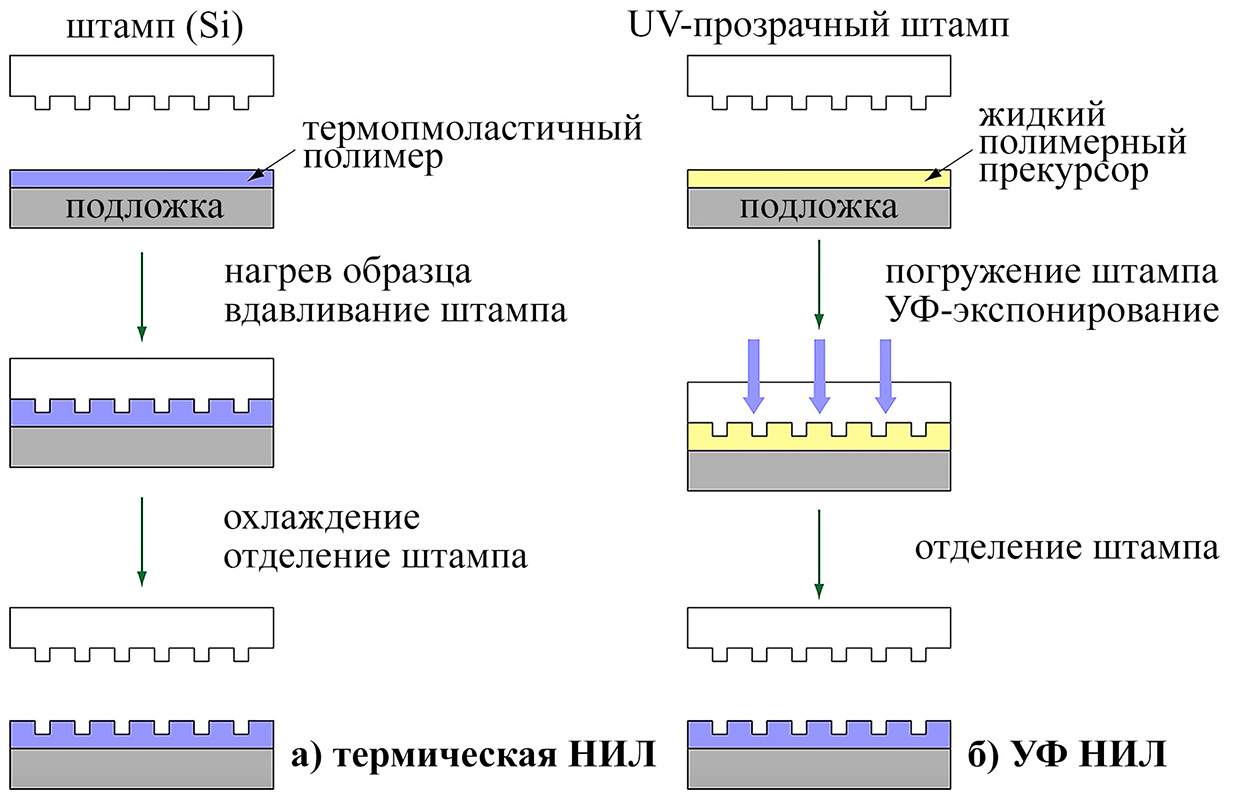
\includegraphics{1_chapter/NIL_14pt_200}
	\vspace{1em}
	\caption{Схематическое изображение метода термической (а) и ультрафиолетовой (б) наноимпринтной литографии.}
	\label{fig:NIL}
\end{figure}


\subsection{Двухфотонная лазерная литография}

Двухфотонная лазерная литография (ДЛЛ) — технология формирования микро- и наноструктур, основанная на двухфотонном поглощении внутри фокального объема лазерного излучения~\cite{Hohmann2015, Kawata2001}. Фотовозбуждение компонент литографической смолы, приводящее к ее отверждению, происходит лишь в окрестности перетяжки сфокусированного лазерного излучения благодаря нелинейному характеру поглощения (рисунок~\ref{fig:TPL}а). Процесс отверждения имеет пороговый характер, что позволяет регулировать размер отверждаемого объема, изменяя дозу или плотность энергии поглощенного лазерного излучения. Последующее погружение смолы в растворитель приводит к удалению тех участков, которые не были подвергнуты воздействию излучения. В качестве источников излучения в ДЛЛ обычно используются фемтосекундные лазеры, работающие в инфракрасном диапазоне, в качестве литографической смолы -- вещество, содержащее реакционно-способные олигомеры и фотоинициатор. При точной фокусировке ДЛЛ способна обеспечить субмикронное разрешение (рисунок~\ref{fig:TPL}б). Поскольку в ДЛЛ положения центров отвреждения могут задаваться произвольно, эта технология нашла применение во многих областях -- микрофлюидике~\cite{TPL_microfluidics_1, TPL_microfluidics_2}, биологии и \linebreak медицине~\cite{TPL_biology_1, TPL_biology_2}, оптике и нанофотонике \cite{TPL_optics, TPL_nanophotonics}, и др. При этом, силу своей природы, данная технология обладает крайне низкой производительностью, что является ее главным недостатком.

\begin{figure}[h]
	\centering
	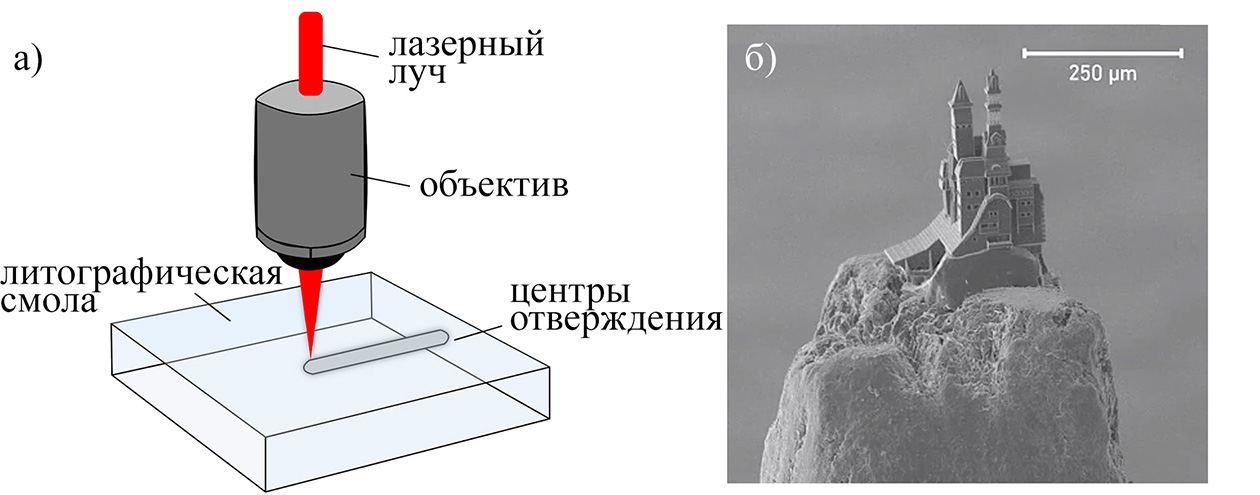
\includegraphics{1_chapter/TPL_14pt_200}
	\vspace{1em}
	\caption{Схематическое изображение метода двухфотонной лазерной литографии (а) и пример структуры, полученной этим методом (б)~\cite{TPL_castle}.}
	\label{fig:TPL}
\end{figure}


\subsection{Интерференционная литография}

Интерференционная литография (ИЛ) -- метод формирования периодической структуры в резисте, основанный на экспонировании резиста пространственно упорядоченным стоячим электромагнитным полем, возникающим при интерференции двух и более когерентных монохроматических или квазимонохроматических пучков излучения~\cite{IL_general} (рисунок~\ref{fig:IL}). Когерентность интерферирующих пучков обычно обеспечивается путем разделения исходного пучка на нужное число вторичных пучков с помощью различных интерференционных схем. В оптическом и УФ-диапазонах используются зеркальные схемы (Френеля, Ллойда и др.), схемы на преломляющей оптике (бипризма Френеля, билинза Бийе) или комбинированные зеркально-линзовые схемы. В этих диапазонах в качестве источника исходного пучка с высокой степенью монохроматичности и когерентности используются лазеры, позволяющие достичь разрешения ИЛ до 100~нм. Вопрос обеспечения более высокого разрешения решается путем перехода в область рентгеновского излучения~\cite{IL_X-ray}. ИЛ применяется для получения  метаматериалов~\cite{IL_metamaterials}, нанофотонных и наноплазмонных устройств~\cite{IL_nanophotonics}, биомедицинских объектов~\cite{IL_biomedical}, изделий на основе выращиваемых наноэлементов и самоорганизующихся структур~\cite{IL_self-assembly} и др. Преимущества метода заключаются в относительной простоте и высокой производительности, к недостаткам можно отнести возможность получения исключительно периодических структур.

\begin{figure}[t]
	\centering
	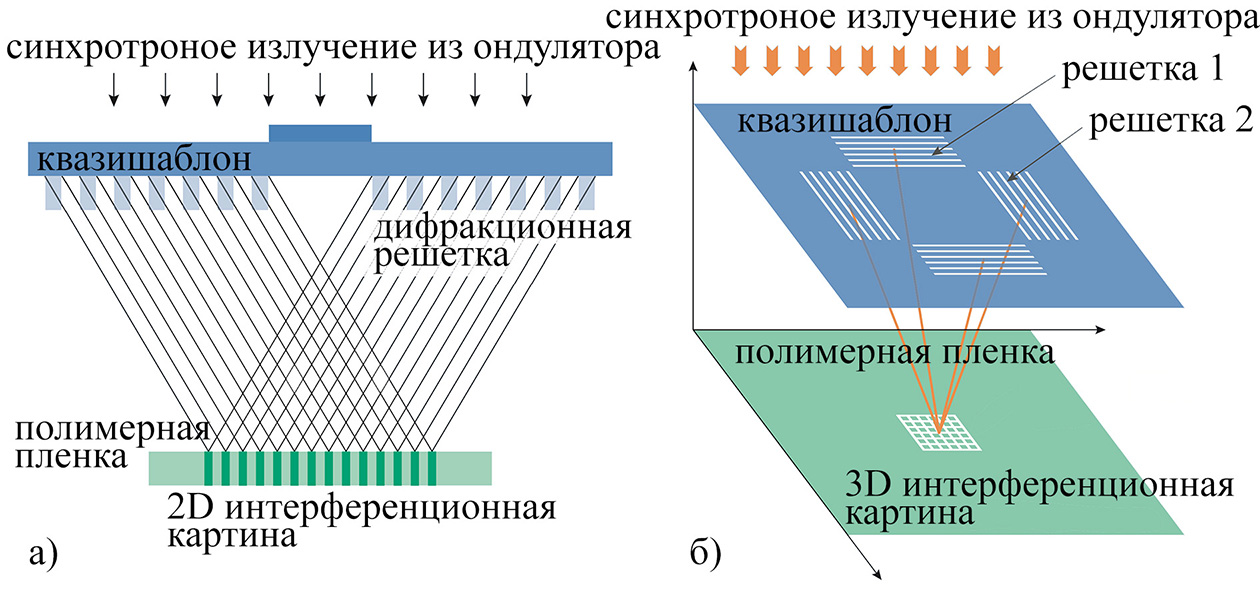
\includegraphics{1_chapter/IL_14pt_200}
	\vspace{0.5em}
	\caption{Схематическое изображение процесса получения двумерных (a) и трехмерных (б) структур методом интерференционной литографии.}
	\label{fig:IL}
\end{figure}


\subsection{Полутоновая литография}

Полутоновая литография (ПЛ) -- общее название для методов, позволяющих получить сложный трехмерный рельеф в литографическом процессе с одной одной стадией экспонирования~\cite{GL_general}. В их основе лежит пространственная модуляция дозы при экспонировании, приводящая к локальному увеличению или уменьшению скорости растворения резиста при проявлении. Таким образом, конечный рельеф, получаемый в резисте, имеет ступенчатую форму и состоит из участков, растворенных в различной степени. Сглаживание границ между участками, проэкспонированных с различными дозами, может быть в дальнейшем достигнуто за счет оплавления образца при температурах вблизи его температуры стеклования (рисунок~\ref{fig:GL}a). При этом такое оплавление может быть использовано как дополнительный этап микроструктурирования~\cite{Kirchner_reflow} (рисунок~\ref{fig:GL}б--г). Таким образом, полутоновая литография с последующим оплавлением образца является гибкой технологией микро- и наноструктурирования, применяемой в оптике и нанофотонике~\cite{GL_optics}, микрофлюидике~\cite{GL_microfluidics}, для формировании микроэлектромеханических систем~\cite{GL_MEMS} и в других областях. Существует как электронно-лучевая, так и фото-ПЛ, однако, фото-ПЛ имеет некоторые ограничения, связанные с оплавлением резиста. Так, например, вязкость широко используемого негативного фоторезиста SU-8 при экспонировании увеличивается, что усложняет процесс его контролируемого оплавления~\cite{Kirchner_GL_review}. Преимущества метода ПЛ заключаются в его универсальности -- варьирование дозы экспонирования и контролируемое оплавление образца позволяют получить практически любой необходимый рельеф. Недостатками метода являются его сложность и производительность, еще более низкая, чем в случае электронно-лучевой литографии.

\begin{figure}[t]
	\centering
	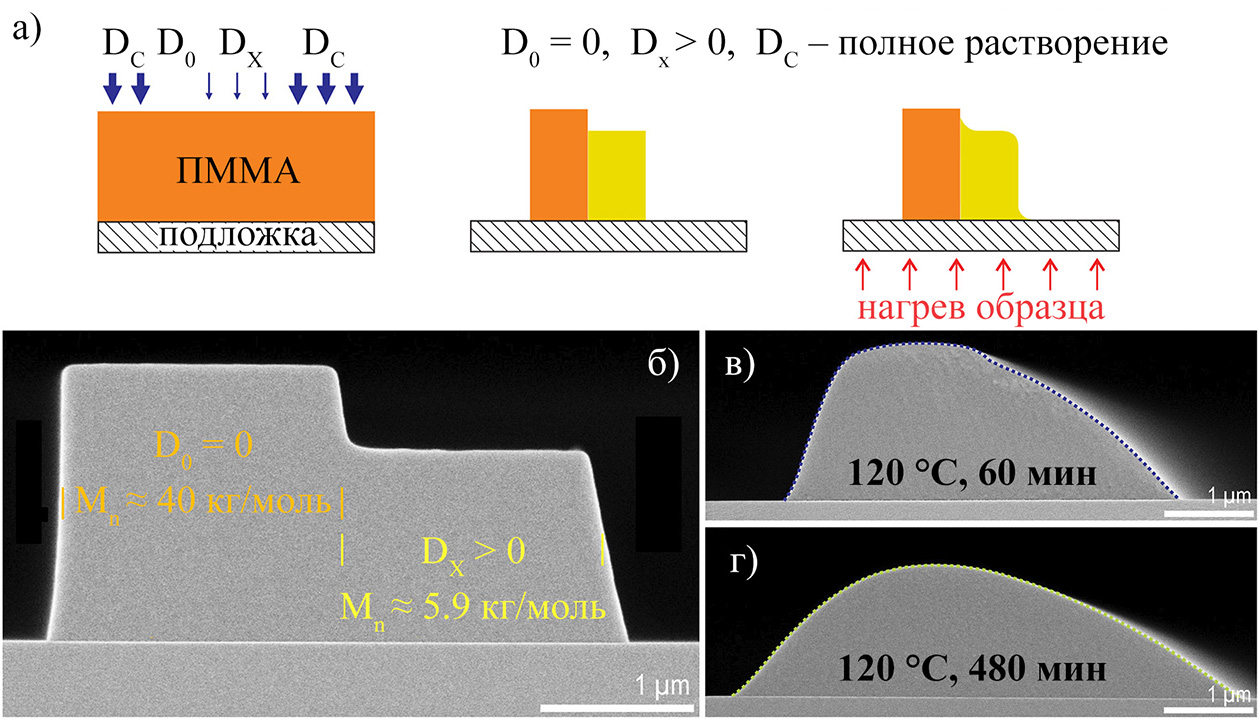
\includegraphics{1_chapter/GL_14pt_200}
	\vspace{1em}
	\caption{Схематическое изображение процесса полутоновой литографии с последующим оплавлением резиста (а) и примеры структуры, полученной в ПММА непосредственно после проявления (б) и при последующем нагреве (в,~г)~\cite{Kirchner_reflow}.}
	\label{fig:GL}
\end{figure}


\subsection{Сканирующая зондовая литография}

Сканирующая зондовая литография (СЗЛ) включает в себя семейство технологий формирования структур с наноразмерным разрешением.
Каждая из технологий основана на применении специального зонда для воздействия на поверхность образца, приводящего к локальным изменениям поверхности.
В зависимости от природы воздействия зонда на поверхность образца можно выделить следующие основные виды СЗЛ:
\begin{itemize}
	\item механическая, в которой изменение поверхности образца происходит в результате механического воздействия зонда~\cite{SPL_mechanical};
	\item  термохимическая, в которой воздействие нагретого зонда на поверхность образца приводит к термической активации различных химических реакций в образце~\cite{SPL_termochemical};
	\item СЗЛ с приложением напряжения, при которой высокая напряженность электростатического поля, создаваемого зондом, приводит к разложению молекул жидкости~\cite{SPL_bias_liquid} или газа~\cite{SPL_bias_gas}, окружающих образец, и локальному отложению материала на образце;
	\item окислительная СЗЛ, основанная на модификации поверхности образца путем ее локального окисления~\cite{SPL_oxidation};
	\item перьевая СЗЛ, в которой сканирующий зонд используется для нанесения на поверхность образца органических, полимерных или коллоидных наночернил~\cite{SPL_dip_pen_1, SPL_dip_pen_2}.
\end{itemize}

Поскольку зонд воздействует только на поверхность образца, этот метод может быть использован только для послойного формирования рельефа (в отличие от, например, ДЛЛ). Однако, высокое разрешение СЗЛ и возможность ее проведения с использованием различных материалов обеспечили ей широкое применение. При этом, как и в случае ДЛЛ, производительность сканирующей зондовой литографии является крайне низкой.


\subsection{Методы на основе термической деполимеризации резиста}

Процесс цепной термической деполимеризации полимерных молекул~\cite{depol_general_1}, обратный процессу полимеризации, может быть использован для формирования рельефа в полимерном резисте.
Цепная термическая деполимеризация резиста может протекать при температурах выше температуры стеклования резиста, и для инициирования этого процесса требуется нарушение целостности главной цепи полимерной молекулы, приводящее к радикализации концов молекулы в месте разрыва~\cite{depol_general_2}.
В процессе цепной термической деполимеризации резиста от полимерной молекулы последовательно отделяется большое число мономеров (по различным данным, от нескольких сотен до нескольких тысяч~\cite{Cowley_1952_1, Mita_PMMA_zip_lengths_T, Inaba_zip_len}), которые вследствие диффузии покидают область, в которой находилась молекула.
Это приводит к появлению свободного пространства в резисте, что и позволяет использовать этот процесс в целях микро- и наноструктурирования.

Существуют два устоявшихся подхода к микроструктурированию на основе цепной термической деполимеризации резиста.
В каждом из них нагревание резиста производится локально, что ограничивает область деполимеризации резиста.
Первый подход по своей сути является термической сканирующей зондовой литографией, в которой для нарушения целостности полимерных молекул используется нагретый зонд~\cite{depol_fabrication_probe}.
Во втором подходе используется сфокусированный лазерный луч, который вызывает локальный нагрев резиста и разрывы в главной цепи его молекул~\cite{depol_fabrication_laser}.

Однако, существует еще один подход, предполагающий нагрев всего слоя резиста, что позволяет цепной реакции термической деполимеризации протекать в любой его области.
На этом подходе основан метод сухого электронно-лучевого травления резиста (СЭЛТР), в котором резист экспонируется электронным лучом при температурах, превышающих температуру стеклования резиста~\cite{Bruk_2016_mee}.
%Отличительными особенностями этого метода является высокая производительность и возможность формирования в резисте дву- и трехмерных структур со скругленным профилем в одностадийном процессе.
%Описанию этого метода будет посвящена вторая часть данной главы.

\section{Сухое электронно-лучевое травление резиста}

Как было отмечено, в существующих методах микро- и нано-структурирования, основанных на термической деполимеризации резиста, нагревание резиста носит локальный характер -- как по времени, так и в пространстве. В отличие от них, в методе СЭЛТР резист остается полностью нагретым на протяжении всего процесса экспонирования. Глобальный характер нагрева резиста приводит к тому, что важным фактором, определяющим конечный профиль линии, становятся процессы термического растекания резиста. Здесь наблюдается определенное сходство с вышеописанным методом полутоновой литографии, дополненным стадией оплавления резиста для сглаживания границ различных участков. Однако, в методе СЭЛТР термическое растекание резиста протекает одновременно со всеми остальными процессами, включающими электронно-стимулированную термическую деполимеризацию резиста и диффузию мономера в слое резиста. Одновременное протекание всех процессов, определяющий конечный профиль линии, получаемой методом СЭЛТР, делает этот метод сложным для теоретического исследования. До настоящего времени метод СЭЛТР исследовался в большей степени экспериментально, и далее будут подробно описаны шаги, предшествовавшие настоящей работе.


\subsection{Цепная термическая деполимеризация полимеров}
В первых работах по изучению термической деполимеризации полимеров проводилось облучение виниловых полимеров ультрафиолетом при температурах выше их температуры стеклования (120--200~$^\circ$C)~\cite{Cowley_1952_1, Cowley_1952_2, Grassie1949_1, Grassie1949_2, Grassie1949_3, Grassie1949_4}. Анализ молекулярно-массового распределения облученных полимеров, получаемого методом гель-проникающей хроматографии, и продуктов распада позволил сделать вывод о цепном характере реакции деполимеризации полимера и получить оценку для средней длины кинетической цепи при деполимеризации. Были определены процессы, протекающие при термической деполимеризации полимеров -- образование активного центра деполимеризации (инициирование кинетической цепи), его распространение вдоль молекулы (рост кинетической цепи) и возможный перенос на другую молекулу, а также затухание активного центра деполимеризации за счет различных эффектов (обрыв кинетической цепи). Были предложены кинетические уравнения, учитывающие данные процессы, что позволило оценить значения констант процессов исходя из экспериментальных данных.

На рисунке~\ref{fig:Cowley_Mn} приведены зависимости отношения среднечисловой молекулярной массы облученного полимера ($\Mn$) к исходной среднечисловой молекулярной массе ($M_\mathrm{n0}$) от степени деградации полимера. Как видно, для образцов высоким значением $M_\mathrm{n0}$ отношение $\Mn / M_\mathrm{n0}$ уменьшается практически линейно, в то время как для образцов с более низким значением $M_\mathrm{n0}$ данное отношение на начальных этапах деградации практически не изменяется. Для обоснования этого явления было выдвинуто предположение о том, что реакция деполимеризации носит цепной характер. Средняя длина кинетической цепи при деполимеризации при этом такова, что длинные молекулы распадаются не до конца, что приводит к изменению $\Mn$. В то же время относительно короткие (относительно средней длины кинетической цепи при деполимеризации) молекулы распадаются полностью, что исключает их вклад в значение $\Mn$.

\begin{figure}[t]
	\centering
	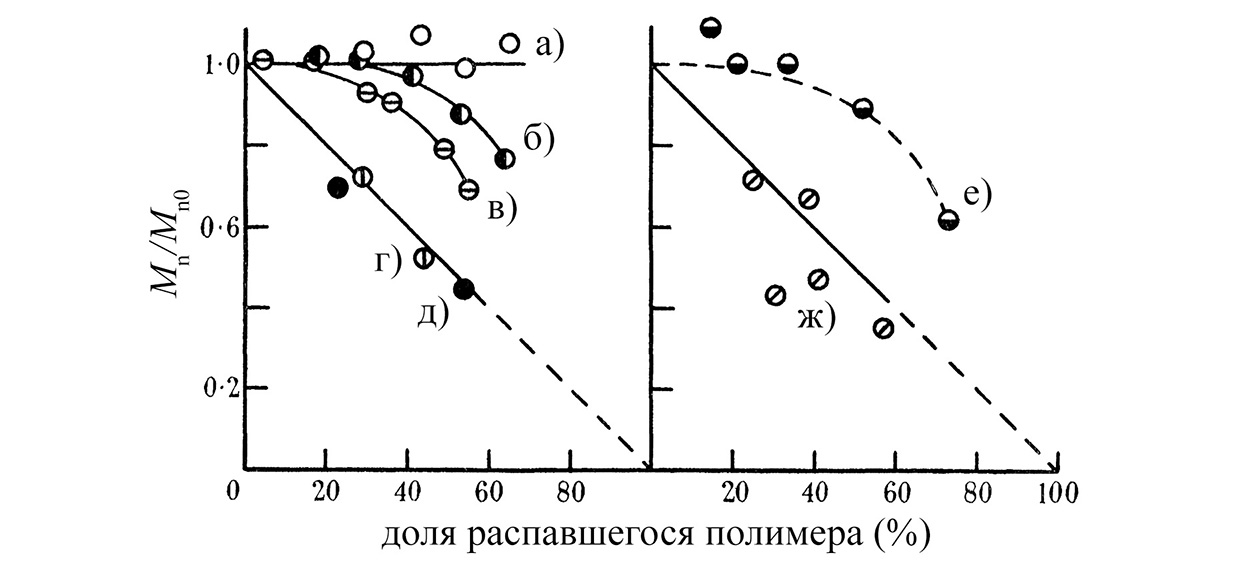
\includegraphics{1_chapter/Cowley_Mn_14pt_200}
	\vspace{0.5em}
	\caption{Зависимости отношения $\Mn / M_\mathrm{n0}$ от доли распавшегося полимера при термической деполимеризации ПММА для различных значений $M_\mathrm{n0}$: a) 44300, б) 94000, в) 179000, г) 650000, д) 725000, е) 125000, ж) 770000~\cite{Cowley_1952_1}.}
	\label{fig:Cowley_Mn}
\end{figure}

Последующие исследования на основе Фурье-спектроскопии позволили более детально описать процесс термической деполимеризации. Так, например, анализ интенсивности отдельных полос спектра, соответствующих различным связям в полимерной молекуле, позволил определить основные механизмы радиационно-стимулированной деполимеризации~\cite{Bermudez} (см. рисунок~\ref{fig:PMMA_degpaths}). В дальнейшем наиболее полная картина процессов термической деполимеризации была сформирована уже за счет применения методов молекулярной динамики~\cite{Stoliarov}.

\begin{figure}[t]
	\centering
	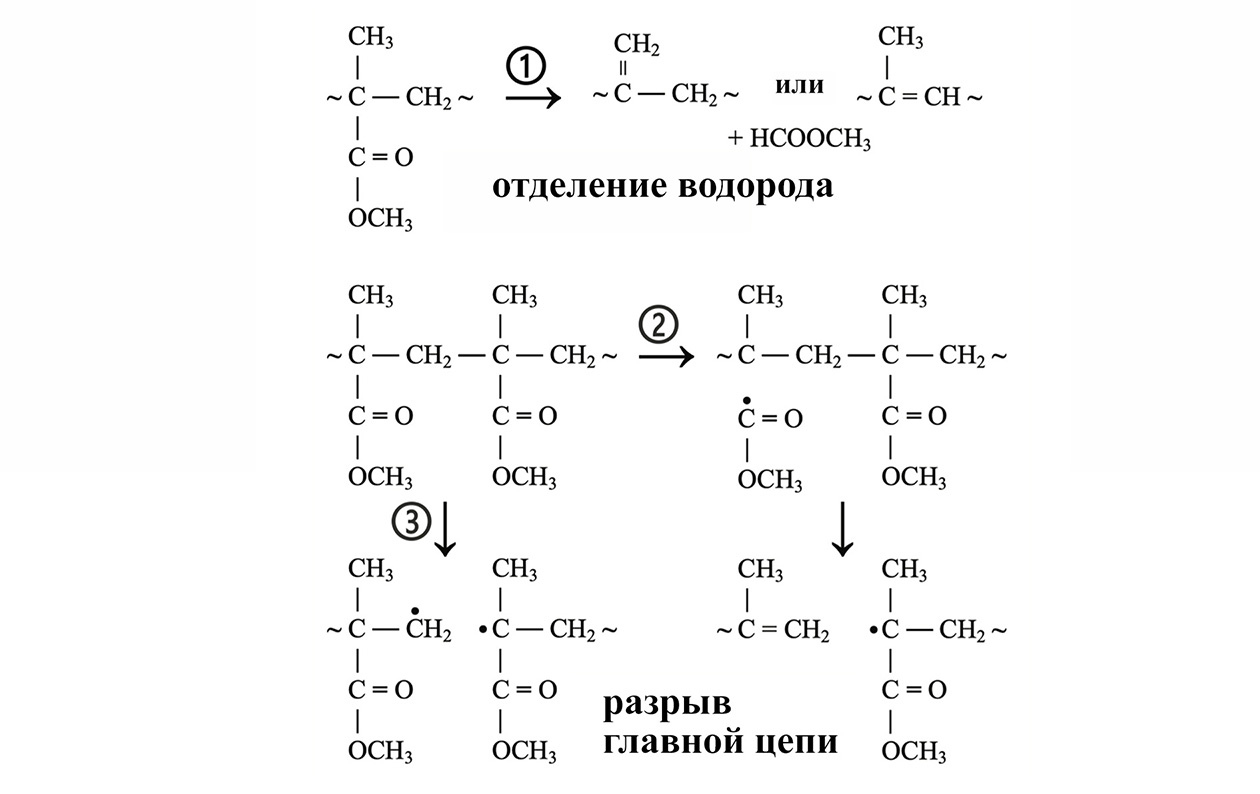
\includegraphics{1_chapter/PMMA_degpaths_14pt_200}
	\caption{Схематическое изображение основных механизмов разрыва молекул ПММА при воздействии внешнего излучения~\cite{Bermudez}.}
	\label{fig:PMMA_degpaths}
\end{figure}

Важной характерной особенностью процесса термической деполимеризации является тот факт, что энергия активации процесса термического образования активного центра деполимеризации превышает энергию активации процесса его распространения вдоль полимерной молекулы~\cite{Cowley_1952_1, Sanchez-Jimenez_Ea}. Это означает, что существует область температур, в которой цепная реакция деполимеризации может протекать только при условии, что активный центр деполимеризации был образован по механизму, отличному от термического. Таким механизмом может являться локальное воздействие внешнего излучения, что приводит к концепции метода микролитографии на основе цепной реакции термической деполимеризации, инициируемой внешним излучением в слое резиста, нагретом до температуры, превышающей температуру стеклования резиста. Первое упоминание о концепции такого метода микролитографии встречается в работе, посвященной ионно-стимулированной термической деполимеризации полиметилметакрилата \linebreak (ПММА)~\cite{Fragala_1}. В последующих работах этого автора была изложена подробная модель образования и выхода мономера из слоя полимера \linebreak (ПММА) при ионно-стимулированной термической деполимеризации~\cite{Fragala_2,Fragala_3_diffusion}, \linebreak однако, к идее метода микролитографии на основе термической деполимеризации он уже не возвращался.


\subsection{Развитие метода микролитографии на основе термической деполимеризации резиста}
Первые шаги в изучении метода микролитографии на основе радиационно-стимулированной термической деполимеризации резиста описываются в работе~\cite{Bruk_2000}. В ней приводятся результаты инициированной $\gamma$-излучением деполимеризации ПММА в виде нанометрового слоя, адсорбированного на поверхности пор силохрома. Несмотря на то, что в данной работе термическая деполимеризация не использовалась для формирования структуры в резисте, а исследовалась в общем, результаты работы позволили определить особенности потенциально возможного метода микроструктурирования на основе этого явления. Так, например, были получены оценки для времени диффузии мономера в слое ПММА после разрушения молекулы и средней длины кинетической цепи при деполимеризации, а также были сделаны выводы о масштабах протекания процессов передачи активного центра деполимеризации на мономер и полимер. Помимо этого было установлено, что при радиационно-стимулированной термической деполимеризации ПММА в области температур 120--180~$^\circ$C влияние процессов реполимеризации пренебрежимо мало.

Впоследствии были проведены эксперименты по изучению термической деполимеризации ПММА, протекающей при его экспонировании электронным лучом, а также впервые были продемонстрированы двумерные и трехмерные структуры, полученные в этом процессе~\cite{Bruk_2013}. Такой метод формирования рельефа в резисте получил название СЭЛТР -- сухое электронно-лучевое травление резиста. Методика экспериментов была следующей:
\begin{enumerate}
	\item На пластину монокристаллического кремния методом ``spin-coating'' из 2\%-ного раствора в анизоле с последующей сушкой наносили слой \linebreak ПММА (PMMA 950K A2 от компании ``Allresist'') толщиной $L_0$ = 80-85~нм;
	\item Полученные образцы помещали на специальный нагреватель, вводили в камеру электронного микроскопа Camscan S-4 или Zeiss Ultra-55, разогревали до нужной температуры и в вакууме порядка 10$^\text{-5}$ мбар подвергали экспонированию электронным лучом в режиме сканирования ``в~кадр'' либо вдоль линии;
	\item После экспонирования нагревательный элемент отключался, и резист остывал в камере электронного микроскопа в вакууме естественным образом;
	\item Толщина слоя резиста до и после процесса СЭЛТР, а также форма получаемого пространственного профиля определялась методом атомно-силовой микроскопии с использованием микроскопа Solver P47-SPM-MTD.
\end{enumerate}

Начальная энергия электронного пучка, ток при экспонировании и диаметр электронного пучка составляли примерно 20 кэВ, 1 нА и 600 нм соответственно для электронного микроскопа Camscan S-4 и 15 кэВ, 1.5 пА и 10 нм соответственно для электронного микроскопа Zeiss Ultra-55.

Одним из важных результатов работы стали кинетические кривые травления в методе СЭЛТР -- зависимости нормализованной толщины слоя резиста $L_\mathrm{norm} = L/L_0$ от дозы экспонирования (рисунок~\ref{fig:kin_curves}). Было установлено, что дозы полутравления $D_\text{0.5}$ (дозы, при которой толщина слоя ПММА уменьшается вдвое относительно начальной толщины) составляют приблизительно 2.5 мкКл/см$\pp$, 0.8 мкКл/см$\pp$ и \linebreak 0.3 мкКл/см$\pp$ для температур 125~$^\circ$С, 150~$^\circ$С и 170~$^\circ$C соответственно. Дозы полного травления слоя резиста $D_\text{1}$ для этих же температур составили приблизительно 20, 12 и 6.5 мкКл/см$\pp$. Таким образом, дозы $D_\text{1}$ примерно в 10 раз (а дозы полутравления -- в 100 раз) меньше доз, необходимых при формировании позитивной маски или рельефа в ПММА методом обычной электронно-лучевой литографии (для которой $D_\text{1}$ составляет порядка 100 мкКл/см$\pp$).

\begin{figure}[t]
	\centering
	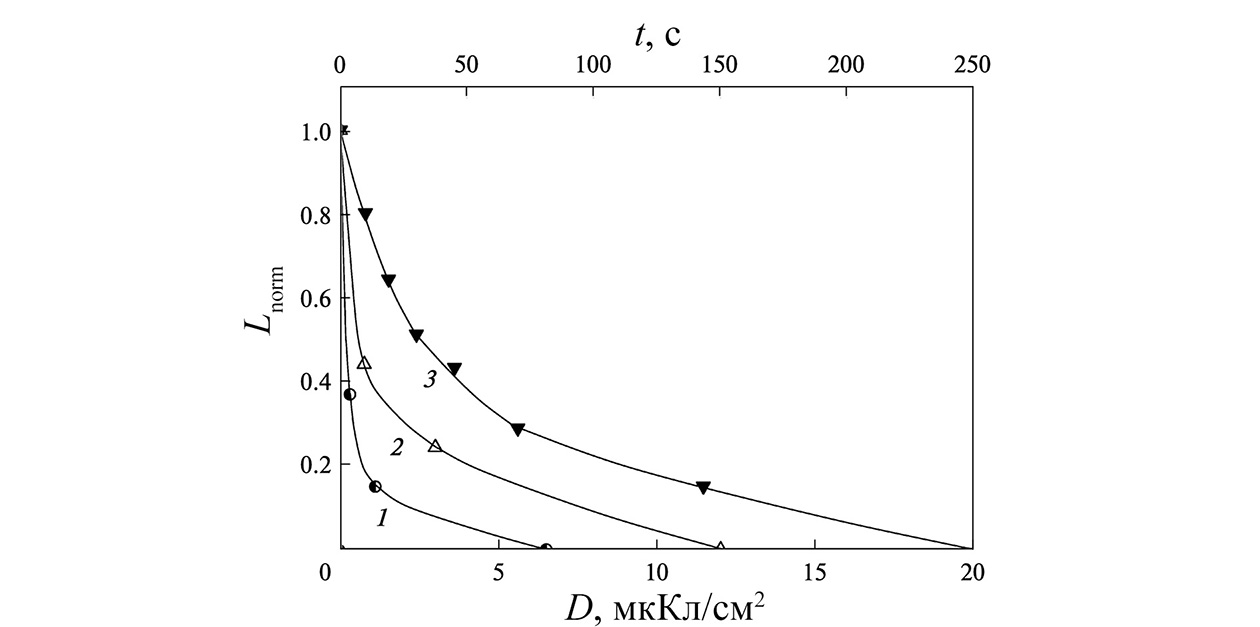
\includegraphics{1_chapter/DEBER_kin_curves_14pt_200}
	\vspace{0.5em}
	\caption{Кинетические кривые травления ПММА в методе СЭЛТР, полученные для температур 125 (1), 150 (2) и 170~$^\circ$С (3)~\cite{Bruk_2013}.}
	\label{fig:kin_curves}
\end{figure}

Было выдвинуто предположение, что в проведенных опытах процесс травления протекал одновременно по всей толщине слоя резиста, а формирование рельефа обеспечивалось объемной релаксацией полимера, которая протекала достаточно быстро по сравнению с характерным временем всего эксперимента. Более того, считалось, что скорость процесса травления являлась приблизительно одинаковой по всей толщине слоя резиста, соответственно, она была пропорциональна текущей толщине слоя ПММА и уменьшается в ходе процесса за счет уменьшения последней. Также предполагалось, что в проведенных опытах диффузия образующегося в слое резиста мономера протекала достаточно быстро для того, чтобы процесс диффузии мономера в газовую фазу не ограничивал скорость травления. Для обоснования этого предположения было введено понятие приведенной скорости травления $W_\mathrm{red}$, которая задается отношением средней скорости травления в некоторой точке кинетической кривой ($V_\mathrm{i}$) к толщине слоя резиста, соответствующей этой точке ($L_\mathrm{i}$):
\begin{equation}
	W_\mathrm{red} = V_\mathrm{i} / L_\mathrm{i}.
\end{equation}

На рисунке~\ref{fig:DEBER_W} приведена зависимость $W_\mathrm{red}$ от нормализованной толщины слоя резиста в ходе процесса СЭЛТР при 125~$^\circ$С. Характер этой зависимости показывает, что даже в начале процесса, когда толщина слоя максимальна, диффузия мономера из слоя резиста протекает достаточно быстро и не влияет на общую скорость травления. В самом деле, если бы диффузия мономера замедляла процесс травления, то $W_\mathrm{red}$ должна была бы возрастать, поскольку время диффузионного проскока молекул газа $\tau_\mathrm{diff}$ пропорционально квадрату толщины слоя $l$, через который происходит диффузия~\cite{Bruk_2000}:
\begin{equation}
	\tau_\mathrm{diff} = l^2 / 12 D,
\end{equation}
где $D$ -- эффективный коэффициент диффузии газа.

\begin{figure}[t]
	\centering
	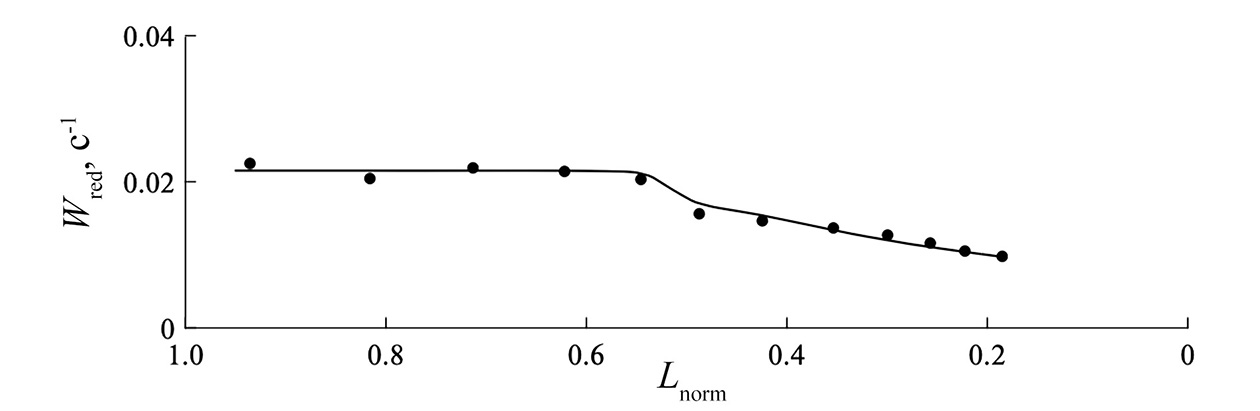
\includegraphics{1_chapter/DEBER_W_14pt_200}
	\vspace{0.2em}
	\caption{Зависимость приведенной скорости травления $W_\mathrm{red}$ для ПММА в методе СЭЛТР при температуре 125 $^\circ$C~\cite{Bruk_2013}.}
	\label{fig:DEBER_W}
\end{figure}

Из рисунка~\ref{fig:DEBER_W} видно, что величина $W_\mathrm{red}$ остается постоянной вплоть до значений конверсии около 50\%, после чего начинает уменьшаться. Наблюдаемое уменьшение $W_\mathrm{red}$ могло быть связано с уменьшением молекулярной массы ПММА и (или) с возникновением в нем в ходе экспонирования дополнительных дефектов, ускоряющих обрыв кинетической цепи при деполимеризации.

Также в работе~\cite{Bruk_2013} были проведены первые опыты по формированию методом СЭЛТР трехмерных ступенчатых структур -- на кремниевой пластине со слоем резиста, разогретыми до необходимой температуры, при неизменном положении пластины производили последовательно несколько экспонирований по последовательно сужающимся квадратным площадкам (рисунок~\ref{fig:DEBER_stairs}). Соотношение линейных размеров площадей сканирования определяло ширину ступеней формирующихся на краю экспонируемой области. Дозы облучения при каждом экспонировании рассчитывались в соответствии с кинетической кривой травления, при этом для каждого последующего экспонирования учитывалась доза, полученная экспонируемой областью ранее. При этом была отмечена достаточно высокая однородность травления по оси $Z$: шероховатость ступенек шириной 5–10 мкм по оси $Z$ составляла всего около 1–2 нм.
Была также отмечена невысокая контрастность получаемого изображения -- угол наклона стенок профиля относительно горизонтали составлял около 3$^\circ$. Было предположено, что основной причиной низкого контраста является специфическая форма кинетической кривой травления в методе СЭЛТР, а также пониженная вязкость ПММА в условиях процесса СЭЛТР, приводящая к растеканию профиля.

\begin{figure}[t]
	\centering
	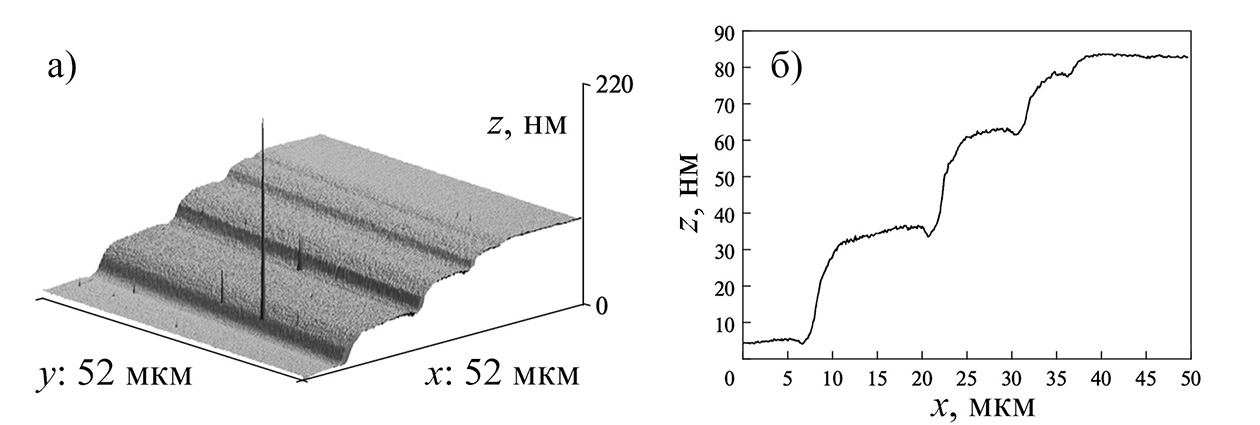
\includegraphics{1_chapter/DEBER_stairs_14pt_200}
	\vspace{0.5em}
	\caption{Ступенчатые профили, полученные в слое ПММА методом СЭЛТР путем экспонирования по последовательно сужающимся квадратным площадкам при температуре 125~$^\circ$C~\cite{Bruk_2013}. \vspace{1.5em}}
	\label{fig:DEBER_stairs}
\end{figure}


\subsection{Текущая стадия разработки метода сухого электронно-лучевого травления резиста}

Наиболее актуальные на сегодняшний день экспериментальные результаты по исследованию метода сухого электронно-лучевого травления резиста приведены в работах~\cite{Bruk_2015_co, Bruk_2016_mee}. Помимо вышеописанных ступенчатых профилей, в этих работах исследовались периодические профили, полученные при экспонировании резиста электронным лучом вдоль серии параллельных линий (рисунок~\ref{fig:DEBER_many_profiles}). Было продемонстрировано, что при таком экспонировании результирующий профиль имеет форму, близкую к синусоидальной, что является аргументом в пользу использования метода СЭЛТР для формирования различных дифракционных и голографических оптических элементов~\cite{Mitreska_sin_gratings}. При этом снова была отмечена высокая производительность метода -- при температуре 160~$^\circ$C полное травление в центре линии было достигнуто при дозе экспонирования менее 1 мкКл/см$\pp$. Также была продемонстрирована возможность достаточно точного переноса профиля, полученного в ПММА, в вольфрам и кремний путем травления в реакторе индуктивно-связанной плазмы (рисунок~\ref{fig:DEBER_Si_W}). За счет этого одной из возможных областей применения метода СЭЛТР может быть формирование штампов для термической НИЛ.

\begin{figure}
	\centering
	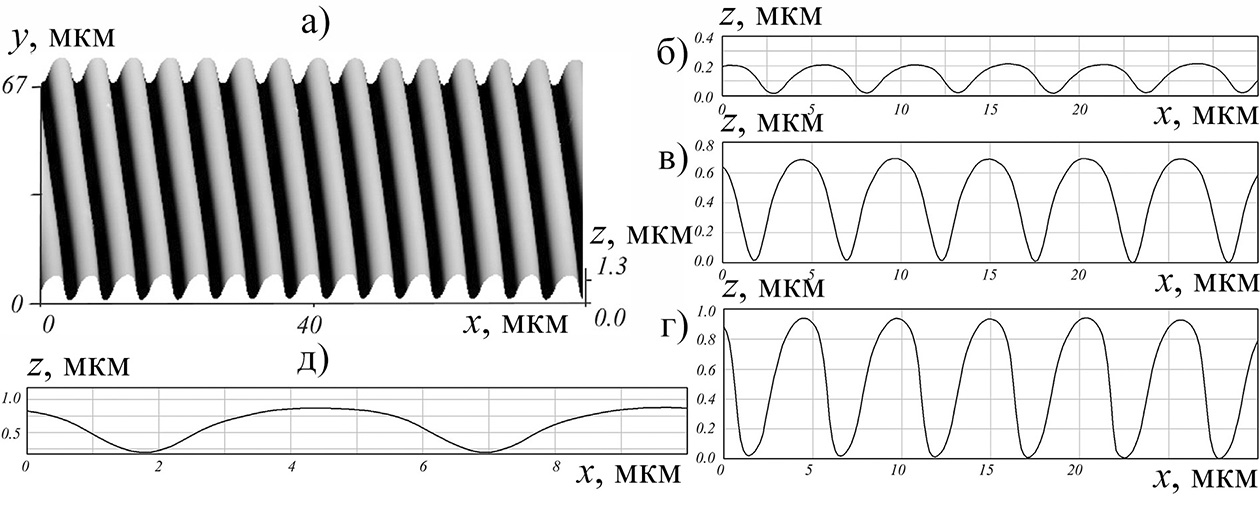
\includegraphics{1_chapter/DEBER_many_profiles_14pt_200}
	\vspace{0.2em}
	\caption{Профили периодических структур, полученных методом СЭЛТР в слое ПММА толщиной 900 нм при экспонировании вдоль серии параллельных линий при температуре 160~$^\circ$C: а) трехмерное изображение; б), в), г) -- профили, полученные при дозах экспонирования 0.05, 0.2 и 0.87 мкКл/см$\pp$ соответственно, д) -- изображение профиля в) в масштабе 1:1~\cite{Bruk_2016_mee}.}
	\label{fig:DEBER_many_profiles}
\end{figure}

\begin{figure}[t]
	\centering
	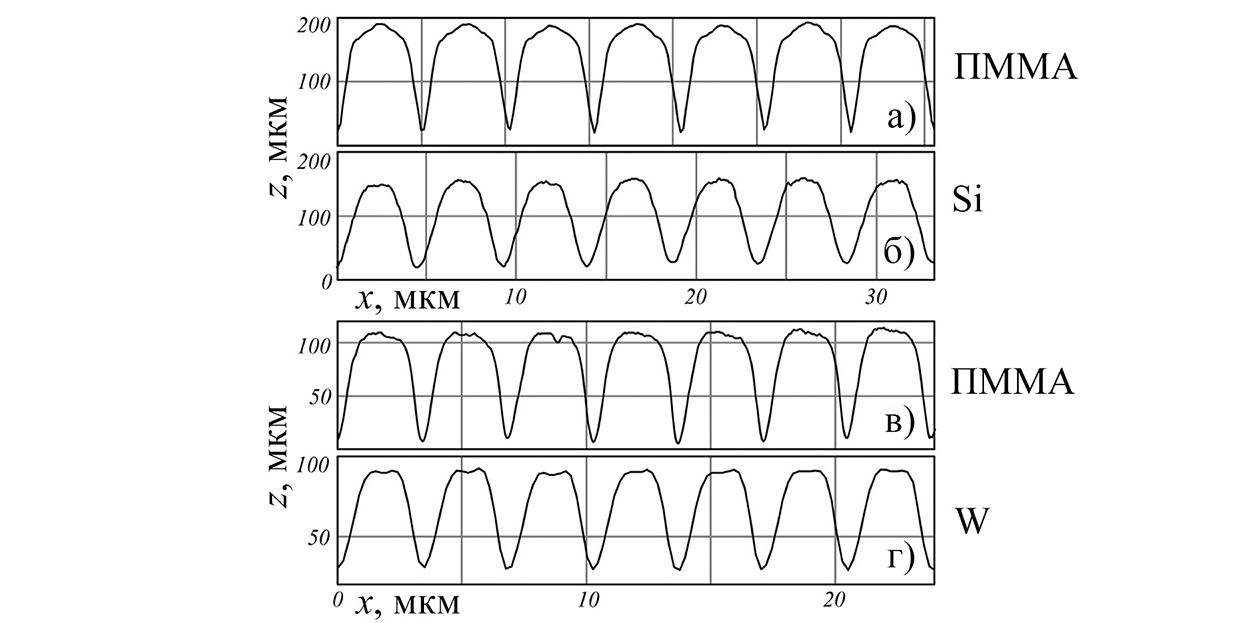
\includegraphics{1_chapter/DEBER_Si_W_14pt_200}
	\vspace{0.2em}
	\caption{Сечения профилей структур, полученных методом СЭЛТР в слое ПММА до (а) и в)) и после (б) и г)) переноса в кремний (Si) и вольфрам (W)~\cite{Bruk_2016_mee}.}
	\label{fig:DEBER_Si_W}
\end{figure}

Для оценки величины латерального разрешения метода СЭЛТР были исследованы профили, полученные при экспонировании резиста остросфокусированным электронным пучком вдоль одиночных линий (рисунок~\ref{fig:DEBER_Ultra}). При диаметре пучка около 10 нм ширина одиночных линий на глубине, равной половине от максимальной глубины травления, составила примерно 300 нм, что было принято за предельное разрешение метода СЭЛТР.

Резюмируя все вышесказанное, можно выделить преимущества и недостатки метода СЭЛТР. К преимуществами данного метода относятся:
\begin{itemize}
	\item высокая производительность метода, обеспечиваемая цепной реакцией термической деполимеризации резиста -- характерные дозы, необходимые для формирования рельефа в резисте методом СЭЛТР в десятки раз меньше, чем характерные дозы при обычной электронно-лучевой литографии;
	\item относительная простота метода -- для формирования дву- и трехмерных структур в резисте требуется всего одна вакуумная стадия;
	\item возможность реализации в различных электронно-лучевых системах -- метод СЭЛТР может быть реализован в растровых электронных микроскопах, электронных литографах и др. электронно-лучевых системах с минимальными модификациями (обеспечение возможности нагрева образца и, при необходимости, установка ловушек для мономера);
	\item сглаженный профиль получаемой структуры, обеспечиваемый процессами растекания.
\end{itemize}

При этом, в настоящее время главными недостатками метода СЭЛТР являются низкие латеральное разрешение и контраст получаемого изображения. До настоящего времени при использовании электронно-лучевых систем с диаметром луча около 10~нм c помощью метода СЭЛТР удавалось получать канавки c минимальной шириной 300-400 нм и максимальным углом наклона стенок около 20$^\circ$. В силу одновременного протекания при СЭЛТР множества различных процессов точный механизм формирования конечного профиля линии не был понятен, что не позволяло выявить пути оптимизации данного метода. Экспериментальные методы исследования процесса СЭЛТР, использовавшиеся до настоящего времени, ограничивались лишь исследованиями конечного профиля получаемых структур. Такой подход не позволяет определить вклад в латеральное разрешение метода СЭЛТР отдельных процессов, что существенно затрудняет его оптимизацию. В то же время, при наличии физической модели метода СЭЛТР, определение путей оптимизации метода и границ его применимости стало бы вполне возможным. Построение такой модели могло бы быть основано на выделении основных процессов, определяющих профиль линии в методе СЭЛТР, разработке их физических моделей на основе существующих подходов и дальнейшем объединении моделей отдельных процессов в общую модель метода, для верификации которой могли бы быть использованы экспериментальные профили.

\begin{figure}
	\centering
	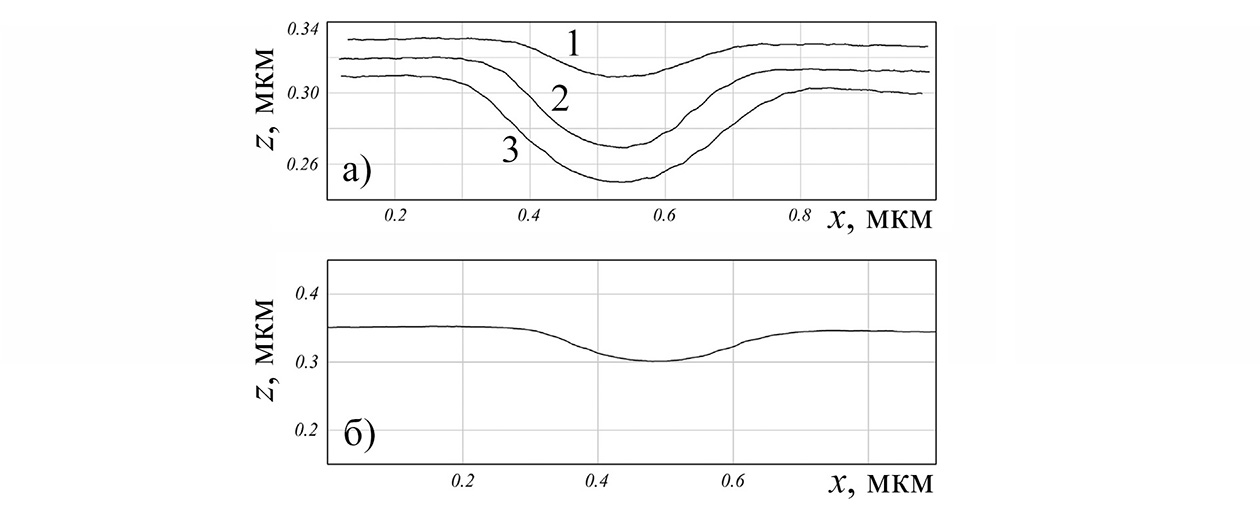
\includegraphics{1_chapter/DEBER_Ultra_14pt_200}
	\caption{а) Профили одиночных линий, полученных методом СЭЛТР в слое ПММА толщиной 80 нм при экспонировании остросфокусированным электронным пучком (диаметр пучка составляет около 10 нм) при температуре 116~$^\circ$C. Время экспонирования составляло 1, 4 и 16 с (профили 1, 2 и 3 соответственно на рисунке); б) Изображение профиля 2 в масштабе 1:1~\cite{Bruk_2016_mee}.}
	\label{fig:DEBER_Ultra}
\end{figure}


Подводя итоги главы, можно выделить несколько важных фактов. Во-первых, в ряде областей является востребованным формирование трехмерных микро- и наноструктур, что осуществляется различными методами, имеющими свои преимущества и недостатки. Во-вторых, исходя из преимуществ и недостатков основных существующих методов 3D микро- и наноструктурирования, можно заключить, что в настоящее время отсутствует метод, который являлся бы одновременно высокопроизводительным и относительно простым в реализации. В-третьих, в качестве такого метода может рассматриваться сухое электронно-лучевое травление резиста (СЭЛТР), однако, недостаточное понимание механизма формирования профиля линии в процессе СЭЛТР существенно затрудняет его применение. Таким образом, целесообразным является построение физической модели метода СЭЛТР, что позволит полностью определить возможности данного метода и оптимизировать его параметры для решения различных задач.
